\documentclass[letterpaper]{article}
\usepackage{arxiv}
\usepackage{natbib}
\setcitestyle{authoryear,square,comma}

%═══════════════════════════════════════════
% Uncomment for debugging and proofreading
%═══════════════════════════════════════════
% \usepackage{lineno}
% \linenumbers

%═══════════════════════════════════════════
% Fonts and math packages
%═══════════════════════════════════════════
\usepackage{times}
\usepackage{helvet}
\usepackage{courier}
\usepackage{bbm}
\usepackage{amssymb,amsthm,amsmath}
\usepackage{mathtools}
\usepackage{proof}
\usepackage{bussproofs}

%═══════════════════════════════════════════
% Formatting, margins, and spacing packages
%═══════════════════════════════════════════
\usepackage{microtype}
%\frenchspacing
% \usepackage{lscape}
\usepackage{setspace}
%\usepackage{fullpage}

%═══════════════════════════════════════════
% Graphics packages
%═══════════════════════════════════════════
\usepackage{tikz}
\usetikzlibrary{positioning,calc,arrows.meta,shapes.geometric,fit}

%═══════════════════════════════════════════
% Environments
%═══════════════════════════════════════════
\usepackage{paralist}
\usepackage{enumitem}
\usepackage{verbatim}
\AtBeginEnvironment{quote}{\par\singlespacing\small}
\setcounter{secnumdepth}{0}
\usepackage{float}
\setlist[description]{leftmargin=1cm,labelindent=1cm}

\usepackage{refcount}
\theoremstyle{definition}
\newtheorem{definition}{Definition}
\newtheorem{theorem}{Theorem}
\newtheorem{lemma}[theorem]{Lemma}
\newtheorem{claim}{Claim}
\newtheorem{corollary}{Corollary}
\newtheorem{proposition}{Proposition}
\newtheorem{example}{Example}
\newtheorem{remark}[theorem]{Remark}

\newtheorem{innercustomthm}{Theorem}
\newtheorem{innercustomdef}{Definition}
\newtheorem{innercustomlemma}{Lemma}
\newtheorem{innercustomcorollary}{Corollary}
\newenvironment{restatetheorem}[1]
  {\renewcommand\theinnercustomthm{#1}\innercustomthm}
  {\endinnercustomthm}
\newenvironment{restatedef}[1]
  {\renewcommand\theinnercustomdef{#1}\innercustomdef}
  {\endinnercustomdef}
\newenvironment{restatelemma}[1]
  {\renewcommand\theinnercustomlemma{#1}\innercustomlemma}
  {\endinnercustomlemma}
\newenvironment{restatecorollary}[1]
  {\renewcommand\theinnercustomcorollary{#1}\innercustomcorollary}
  {\endinnercustomcorollary}

%═══════════════════════════════════════════
% References, Links, and Color
%═══════════════════════════════════════════
\usepackage{hyperref}
\definecolor{myblue}{rgb}{0.03, 0.27, 0.65}
\definecolor{myred}{rgb}{0.82, 0.1, 0.26}
\hypersetup{
    colorlinks=true,
    linkcolor=myblue,
    urlcolor=myblue,
    citecolor=myblue,
}
\urlstyle{same}

\usepackage{xcolor}
\definecolor{myblue1}{RGB}{158,202,225}
\definecolor{myblue2}{RGB}{49,130,189}

%═══════════════════════════════════════════
% Custom Commands, General Use
%═══════════════════════════════════════════
\newcommand{\Set}{\mbox{\sf Set}} 
\newcommand{\semantics}[1]{[\![\mbox{\em $ #1 $\/}]\!]}
\newcommand{\Model}{\mathcal{M}}
\newcommand{\Nodel}{\mathcal{N}}
\newcommand{\lang}{\mathcal{L}}
\newcommand{\vocab}{\mathcal{V}}
\newcommand{\wocab}{\mathcal{W}}
\newcommand{\set}[1]{\{ #1 \}}
\newcommand{\proves}{\vdash}
\renewcommand{\o}{\cdot}
\newcommand{\orr}{\vee}
\newcommand{\andd}{\wedge}
\newcommand{\nott}{\neg}
\newcommand{\bigandd}{\bigwedge}
\newcommand{\quadiff}{\quad \mbox{ iff } \quad}
\newcommand{\rem}[1]{\relax}
 \newcommand{\NP}{\mbox{\sc np}}
\newcommand{\axiom}{\textsc}
\newcommand*{\bigchi}{\mbox{\Large$\chi$}}% big chi

%═══════════════════════════════════════════
% Custom Commands, Hebbian Learning
%═══════════════════════════════════════════
\newcommand{\Typ}{\textrm{\textup{\textbf{T}}}}
\newcommand{\Prop}{\textsf{Prop}}
\newcommand{\Update}{\textsf{Update}}
\newcommand{\Inc}{\textsf{Hebb}}
\newcommand{\AllNets}{\mathsf{Net}}
\newcommand{\Net}{\mathcal{N}}

%═══════════════════════════════════════════
% Title, Author, Pdfinfo
%═══════════════════════════════════════════
\hypersetup{pdfinfo={
Title={The Logic of Hebbian Learning},
Author={Caleb Kisby, Sa\'{u}l A. Blanco, Lawrence S. Moss},
Keywords={Neurosymbolic AI, Hebbian Learning,
Dynamic Logics, Knowledge Representation and Reasoning, Nonmonotonic Reasoning, Preference Upgrade}
}}

\renewcommand{\headeright}{}
\renewcommand{\undertitle}{}

\title{The Logic of Hebbian Learning}
\author{\textbf{Caleb Kisby$^1$, Sa\'{u}l A. Blanco$^1$, Lawrence S. Moss$^2$}\\
\normalsize $^1$Department of Computer Science, Indiana University\\ 
\normalsize $^2$Department of Mathematics, Indiana University\\
\normalsize Bloomington, IN 47408, USA\\
\normalsize \{cckisby, sblancor, lmoss\}@indiana.edu}
% \and
% Lawrence S. Moss \\
% Department of Mathematics, Indiana University,\\ Bloomington, IN 47405, USA\\
% lmoss@indiana.edu}
\date{}

%═══════════════════════════════════════════
% Beginning of Paper
%═══════════════════════════════════════════
 \begin{document}
\maketitle

\vspace*{-2\baselineskip}
\setlength{\fboxrule}{0.8pt}
\setlength{\fboxsep}{1em}
\begin{center}
\fbox{\parbox{\linewidth-(\linewidth/3)}{

\textbf{Note:} This arXiv print is a fuller version of our FLAIRS paper \citep{kisby2022logic}, complete with proofs we could not include in the conference format.  We have also corrected a couple of errors, as well as certain aesthetic choices that made the proof system somewhat awkward. Otherwise, we have kept as close to the original as possible; for a more up-to-date version of the system presented here, see our follow-up work \citep{kisby2024hebbian}.
}}
\end{center}
\vspace*{2\baselineskip}

\begin{abstract}
We present the logic of Hebbian learning, a dynamic logic whose semantics\footnote{A Python implementation of our semantics, using Tensorflow \& Keras \citep{tensorflow2015-whitepaper}), is available at
\center{\url{https://github.com/ais-climber/neural-semantics}}}
are expressed in terms of a layered neural network learning via Hebb's associative learning rule.  Its language consists of modality $\Typ \varphi$ (read ``typically $\varphi$,'' formalized as forward propagation), conditionals $\varphi \Rightarrow \psi$ (read ``typically $\varphi$ are $\psi$''), as well as dynamic modalities $[\varphi^+] \psi$ (read ``evaluate $\psi$ after performing Hebbian update on $\varphi$'').  We give axioms and inference rules that are sound with respect to the neural semantics; these axioms characterize Hebbian learning and its interaction with propagation.  The upshot is that this logic describes a neuro-symbolic agent that both learns from experience and also reasons about what it has learned.
\end{abstract}

%═══════════════════════════════════════════
\section{Introduction}
%═══════════════════════════════════════════

Artificial intelligence  has  long  been  marked  by  a  schism between two of its major paradigms: symbolic reasoning and connectionist learning.  Neural systems have had wild success with learning from unstructured data, whereas symbolic reasoners are notorious for their rigidity.  On the other hand, symbolic systems excel at sophisticated (static) reasoning tasks that neural systems cannot readily learn.  Symbolic systems also tend to have more explainable reasoning, thanks to their use of explicit inferences in an intuitive language.  Moreover, due to their connection with logic, it is straightforward to compare the relative power and complexity of different symbolic reasoners.

But as Valiant famously put it, intelligent cognitive agents must have \emph{both} ``the ability to learn from experience, and the ability to reason from what has been learned'' \citep{valiant2003three}.  \emph{Neuro-symbolic artificial intelligence} has emerged in the last few decades to address this challenge --- a monumental effort to integrate neural and symbolic systems, while retaining the advantages of both (see \citep{bader2005dimensions} and \citep{sarker2021neuro}, two surveys that span the decades).  Despite the cornucopia of neuro-symbolic proposals, the field has not yet agreed on an interface between the two that satisfyingly preserves both flexible learning and expressive reasoning.

Following the path set out by \citep{balkenius1991nonmonotonic} and \citep{leitgeb2001nonmonotonic,leitgeb2003nonmonotonic}, we advance the following proposal for the neuro-symbolic interface.  Rather than viewing the neural and symbolic as two different systems to be combined, we view them as two ways of interpreting the same agent.  More precisely, we view the dynamics of neural networks as the semantics to a formal logic.  This logic serves as a bridge between the neural network model and formal inference.

Previous work, particularly \citep{leitgeb2001nonmonotonic}, has considered how forward propagation in binary feed-forward nets forms a sound and complete semantics for the (static) conditional logic \textbf{CL} (\emph{loop-cumulative}).  The novelty of our paper is that we extend this logic by viewing a simple learning policy --- Hebbian update (``neurons that fire together wire together'') --- as a dynamic modality.  By doing so, we demonstrate that the dynamics of Hebbian learning (in binary feed-forward nets) directly corresponds to a particular dynamic multimodal logic that we call \emph{the logic of Hebbian learning}.
This logic meets Valiant's challenge:  It characterizes a cognitive agent that can learn from experience and also reason about what it has learned.

Our main result is the soundness of axioms and inference rules that characterize Hebbian learning.  The most interesting axioms involve the interaction between Hebbian update and forward propagation.  We also demonstrate how our logic models the learning of a concrete neural network. And although we leave the question of completeness open, we close by considering the importance of completeness for logics of this kind.

%═══════════════════════════════════════════
\section{Related Work}
%═══════════════════════════════════════════

\subsubsection{Logics with Neural Semantics.}
%═══════════════════════════════════════════
The idea that we can view neural networks as the semantics for symbolic reasoning dates back to \citep{mcculloch1943logical}.  Our work builds on a recent reimagining of this \`a la \citep{balkenius1991nonmonotonic}, \citep{leitgeb2001nonmonotonic,leitgeb2003nonmonotonic,leitgeb2018neural}, which formally characterize the dynamics of inhibitory neural networks as conditional logics.  Similarly, \citep{blutner2004nonmonotonic} demonstrates that Hopfield networks correspond to the logic of what he calls ``weight-annotated Poole systems.''  More recently, \citep{giordano2021} describe multilayer perceptrons and self-organizing maps in terms of defeasible description logics.  Yet no neural semantics to date has tackled the issue of learning --- doing this for Hebbian learning is precisely the contribution of our paper.

\subsubsection{Neuro-Symbolic AI.}
%═══════════════════════════════════════════
Across the neuro-symbolic literature, an ubiquitous premise is that integration involves combining or composing otherwise distinct neural and symbolic modules.  In contrast, this paper presents the neural and symbolic as two perspectives we can have about the same agent.

To our knowledge, the combined work of \citep{garcez2001symbolic} and \citep{garcez2008neural} is the only neuro-symbolic proposal (besides neural semantics, see above) that exhibits this intimate interface between the two.  The former gives a formally sound method for extracting conditionals from a network and the latter gives a method for build neural network models from rules (in a variety of different logics).  When combined, we can freely translate between a neural network and its beliefs.  But unlike our work, this framework does not offer a logical account of the neural network's learning.

% SAVE FOR JOURNAL VERSION
%Consider Henry Kautz' recent taxonomy of neuro-symbolic systems \citep{kautz-2020future}: All five of his categories involve combining or composing otherwise distinct neural and symbolic modules.

\subsubsection{Dynamic Logics for Learning.}
%═══════════════════════════════════════════
Two recent papers, \citep{baltag2019dynamic} and \citep{baltag2019right}, also present dynamic multimodal logics that characterize learning.  The former models an individual's learning in the limit, whereas the latter models supervised learning as a game played between student and teacher.  But it is unclear how learning policies expressed in these logics might relate to specific neural implementations of learning such as Hebbian update and backpropagation.

Furthermore, the syntax and inferences of our logic do not resemble either of these in a meaningful way. Perhaps the closest logics to ours are dynamic logics of \emph{preference upgrade}, in the sense of \citep{van2007prefupgrade}.  In particular, consider the modalities $[{\Uparrow} \varphi]$ (lexicographic upgrade) and $[{\uparrow} \varphi]$ (elite change) \citep{van2007beliefrevision}.  Both of these operators implement policies for modifying an agent's preference relation $<$ over possible worlds.  As with our logic, the key axioms characterizing these policies deal with their interaction with conditionals $\varphi \Rightarrow \psi$.  But the semantics of our logic are very different; we leave the issue of how our neural semantics relate to classical preference relations to future work.  In addition, both $[{\Uparrow} \varphi]$ and $[{\uparrow} \varphi]$ are reducible to the static language of conditionals, whereas it is presently unclear how our $[\varphi^+]$ might reduce to its base language.


%═══════════════════════════════════════════
\section{Background}
%═══════════════════════════════════════════

\subsection{Neural Network Models}
%═══════════════════════════════════════════

A model of the logic of Hebbian learning is just a special type of artificial neural network that we call a \emph{binary feedforward neural network} (BFNN).

\begin{definition} A BFNN is a pointed directed graph ${\Net = \langle N, E, W, A, O, \eta \rangle}$, where
\begin{itemize}
    \item $N$ is a finite nonempty set (the set of neurons)
    \item $E \subseteq N \times N$ (the set of excitatory connections)
    \item $W : N \times N \to \mathbb{R}$ (the weight of a given connection)
    
    \item $A$ is a function which maps each $n \in N$ to
    $A^{(n)} : \mathbb{R}^k \to \mathbb{R}$ (the activation function for $n$, where $k$ is the indegree of $n$)
    \item $O$ is a function which maps each $n \in N$ to 
    $O^{(n)} : \mathbb{R} \to \set{0, 1}$ (the output function for $n$)
    \item $\eta \in \mathbb{R}, \eta \geq 0$ (the learning rate)
\end{itemize}
As shorthand, we sometimes write $W_{ij}$ to mean $W(i,j)$, for ${(i, j) \in E}$. Moreover, BFNNs are \emph{feed-forward}, i.e. they do not contain cycles of edges with all nonzero weights.  BFNNs are also \emph{binary}, i.e. the output of each neuron is in $\set{0, 1}$.  This binary assumption is unrealistic in practice, although letting it go is just a matter of extending our two-valued logic towards a fuzzy-valued logic (left to future work).

We further require that each composition of activation and output functions ${O^{(n)} \circ A^{(n)}}$ is \textit{strictly} monotonically increasing, i.e. for all $\vec{x}, \vec{y} \in \mathbb{R}^k$ if $\vec{x} < \vec{y}$ then $O^{(n)}(A^{(n)}(\vec{x})) < O^{(n)}(A^{(n)}(\vec{y}))$.  We will more often refer to the equivalent condition:
\begin{equation}\tag{$\ast$}
\label{eqn:increasing}
\vec{x} \leq \vec{y} \quad \mbox{ iff } \quad  O^{(n)}(A^{(n)}(\vec{x})) \leq O^{(n)}(A^{(n)}(\vec{y}))
\end{equation}
Our activation functions include in particular those sigmoid functions commonly used for neural networks in practice.
\end{definition}

% We write $W_{ij}$ to mean $W(i,j)$, for ${(i, j) \in E}$.  

% When $m_i$ is drawn from a sequence ${m_1, \ldots, m_k}$, we write $\overrightarrow{W}(m_i, n)$ as shorthand for the sequence $W(m_1, n), \ldots, W(m_k, n)$.


\subsection{The Dynamics of Propagation}
%═══════════════════════════════════════════

Of course, BFNNs are not merely static directed graphs, but are dynamic in nature.  When a BFNN receives a signal (which we model as the initial state), it propagates that signal forward until the state of the net stabilizes.  This stable state of the net is considered to contain the net's response (answer) to the given signal (question).  We model forward propagation as follows, drawing heavily from the approach proposed by \citep{leitgeb2001nonmonotonic}.

We consider a neuron $n$ active if its activation $A^{(n)}$ is high enough to trigger an output $O^{(n)}$ of $1$ (intuitively, if the neuron fires).  Since our BFNNs are binary, either a given neuron is active ($1$) or it is not ($0$).  So we can identify the state of $\Net$ with the set of neurons that are active.  For a given BFNN $\Net$, let its set of states be
\[
    \Set = \set{S \mid S \subseteq N}
\]
We can get the activation value of a particular neuron in a state $S$ using the following characteristic function:
\begin{definition}
    For $S \in \Set$, let 
    $\bigchi_S : N \to \set{0, 1}$ be given by $\bigchi_S(n) = 1$ iff $n \in S$
\end{definition}

Neurons in a state $S \in \Set$ can subsequently activate new neurons, which activate yet more neurons, until eventually the state of $\Net$ stablizes.  We call this final state of affairs $\Prop(S)$, the \emph{propagation} of $S$.

\begin{definition}
\label{def:propagation}
Let $\Prop : \Set \to \Set$ be defined recursively as follows:  $n \in \Prop(S)$ iff either
Let $\Prop : \Set \to \Set$ be defined recursively as follows:  $n \in \Prop(S)$ iff either
\begin{description}
    \item[(Base Case)] $n \in S$, or
    \item[(Constructor)] The weighted sum of predecessors of $n$ subsequently activate it; for those $m_1, \ldots, m_k$ such that $m_i{E}n$ we have
    \[
    O^{(n)}(A^{(n)}(\sum_{m_i{E}n} W(m_i, n) \cdot \bigchi_{\Prop(S)}(m_i))) = 1
    \]
\end{description}
\end{definition}

Alternatively, consider a finite automaton with state space $\Set$ and transition function $F_{S^\ast} : \Set \to \Set$ tracking the propagation of an initial state $S^\ast$ through $\Net$.  We can view $\Prop(S^\ast)$ as a fixed point of $F_{S^\ast}$ \citep{leitgeb2001nonmonotonic}.
% Leitgeb claims that Prop(S*) is *the unique* fixed point.  I'd like to be able to say this, but I should prove it myself for BFNNs.

The following theorem, due to \citep{leitgeb2001nonmonotonic}, says that we can neatly characterize the algebraic structure of $\Prop$ as a closure operator. Note that Leitgeb proves this for \emph{inhibition nets}, i.e. weightless BFNNs with both excitatory and inhibitory connections. But inhibition nets and our BFNNs are equivalent with respect to their propagation structure --- we prove this result again for BFNNs as a kind of ``sanity check'' that our definitions are correct.

\begin{theorem}
\label{thm:prop-props}
Let $\Net \in \AllNets$.  For all $S, S_1, S_2 \in \Set$, $\Prop$ satisfies
\begin{description}
    \item[(Inclusion)] $S \subseteq \Prop(S)$
    
    \item[(Idempotence)] $\Prop(S) = \Prop(\Prop(S))$
    
    \item[(Cumulative)] If ${S_1 \subseteq S_2 \subseteq \Prop(S_1)}$ then ${\Prop(S_1) = \Prop(S_2)}$
    
    \item[(Loop)] If ${S_1 \subseteq \Prop(S_0)}, \ldots, {S_k \subseteq \Prop(S_{k-1})}$ and ${S_0 \subseteq \Prop(S_k)}$,\\ then ${\Prop(S_i) = \Prop(S_j)}$
    for all $i, j \in \set{0, \ldots, k}$
\end{description}
\end{theorem}
\begin{proof} We prove each in turn:
\begin{description}
    %═══════════════════════════════════════════
    \item[(Inclusion)] If $n \in S$, then $n \in \Prop(S)$ by the base case of $\Prop$.
    
    
    %═══════════════════════════════════════════
    \item[(Idempotence)] The $(\subseteq)$ direction is just Inclusion.  As for $(\supseteq)$, let $n \in \Prop(\Prop(S))$, and proceed by induction on $\Prop(\Prop(S))$.
    
    \begin{description}
    \item[Base Step:] $n \in \Prop(S)$, and so we are done.
    
    \item[Inductive Step:] Let $m_1, \ldots, m_k$ be the predecessors of $n$. We have
    \[
    O^{(n)}(A^{(n)}(\sum_{m_i{E}n} W(m_i, n) \cdot \bigchi_{\Prop(\Prop(S))}(m_i))) = 1
    \]
    By inductive hypothesis, each $m_i \in \Prop(\Prop(S))$ iff $m_i \in \Prop(S)$, and so
    \[
    O^{(n)}(A^{(n)}(\sum_{m_i{E}n} W(m_i, n) \cdot \bigchi_{\Prop(S)}(m_i))) = 1
    \]
    By definition, this means that $n \in \Prop(S)$.
    \end{description}
    
    
    %═══════════════════════════════════════════
    \item[(Cumulative)] For the $(\subseteq)$ direction, let $n \in \Prop(S_1)$.  We proceed by induction on $\Prop(S_1)$.
    
    \begin{description}
    \item[Base Step:] $n \in S_1$.  Well, $S_1 \subseteq S_2 \subseteq \Prop(S_2)$, so $n \in \Prop(S_2)$.
    
    \item[Inductive Step:] Let $m_1, \ldots, m_k$ be the predecessors of $n$. We have
    \[
    O^{(n)}(A^{(n)}(\sum_{m_i{E}n} W(m_i, n) \cdot \bigchi_{\Prop(S_1)}(m_i))) = 1
    \]
    By inductive hypothesis, each $m_i \in \Prop(S_1)$ iff $m_i \in \Prop(S_1)$, and so
    \[
    O^{(n)}(A^{(n)}(\sum_{m_i{E}n} W(m_i, n) \cdot \bigchi_{\Prop(S_2)}(m_i))) = 1
    \]
    By definition, this means that $n \in \Prop(S_2)$.
    \end{description}
    
    Now consider the $(\supseteq)$ direction.  The Inductive Step holds similarly (just swap $S_1$ and $S_2$).  As for the Base Step, if $n \in S_2$ then since $S_2 \subseteq \Prop(S_1)$, $n \in S_1$.
    
    
    %═══════════════════════════════════════════
    \item[(Loop)] Let $k \geq 0$ and suppose the hypothesis.  Our goal is to show that for each $i$, $\Prop(S_i) \subseteq \Prop(S_{i-1})$, and additionally $\Prop(S_0) \subseteq \Prop(S_k)$.  This will show that all $\Prop(S_i)$ contain each other, and so are equal.  Let $i \in \set{0, \ldots, k}$ (if $i = 0$ then $i-1$ refers to $k$), and let $n \in \Prop(S_i)$.  We proceed by induction on $\Prop(S_i)$.
    
    \begin{description}
    \item[Base Step:] $n \in S_i$, and since $S_i \subseteq \Prop(S_{i-1})$ by assumption, $e \in \Prop(S_{i-1})$.
    
    \item[Inductive Step:] Let $m_1, \ldots, m_k$ be the predecessors of $n$. We have
    \[
    O^{(n)}(A^{(n)}(\sum_{m_i{E}n} W(m_i, n) \cdot \bigchi_{\Prop(S_i)}(m_i))) = 1
    \]
    By inductive hypothesis, each $m_i \in \Prop(S_i)$ iff $m_i \in \Prop(S_{i-1})$, and so
    \[
    O^{(n)}(A^{(n)}(\sum_{m_i{E}n} W(m_i, n) \cdot \bigchi_{\Prop(S_{i-1})}(m_i))) = 1
    \]
    By definition, this means that $n \in \Prop(S_{i-1})$. \qedhere
    \end{description}
\end{description}
\end{proof}


%-------------------------------------------------------
%-------------------------------------------------------
\begin{figure}
\centering{
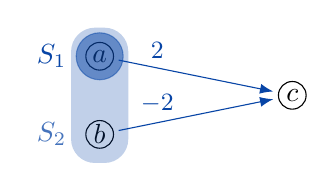
\begin{tikzpicture}[loose/.style={inner sep=.7em},edge/.style = {->,-Latex},
oval/.style={ellipse,draw}]

% nodes
\node[circle,minimum size=10pt,inner sep=0pt,outer sep=2pt,fill=white,draw](a){$a$};
\node[below=0.5 of a,circle,minimum size=10pt,inner sep=0pt,outer sep=2pt,fill=white,draw](b){$b$};

\node[right=2.2 of $(a)!0.5!(b)$,circle,minimum size=10pt,inner sep=0pt,outer sep=2pt,fill=white,draw](c){$c$};

% sets
\node[fill=myblue,color=myblue, opacity=0.5,oval,fit=(a),inner sep=-1pt]{};
\node[fill=myblue, opacity=0.25,rectangle,rounded corners=2ex,fit=(a) (b)]{};
% \node[fill=myblue, opacity=0.25,rectangle,rounded corners=2ex,fit=(c)]{};

% set labels
\node [color=myblue,opacity=1,left=0.3 of $(a)$]{$S_1$};
\node [color=myblue,opacity=0.75,left=0.3 of $(b)$]{$S_2$};
% \node [color=myblue,opacity=0.75,above=0.3 of $(c)$]{flies};

\draw[edge, color=myblue] (a) -- (c) node [near start, above] {\small{\textbf{$2$}}};
\draw[edge, color=myblue] (b) -- (c) node [near start, above] {\small{\textbf{$-2$}}};
\end{tikzpicture}
%-------------------------------------------------------
\hspace{2 cm}
%-------------------------------------------------------
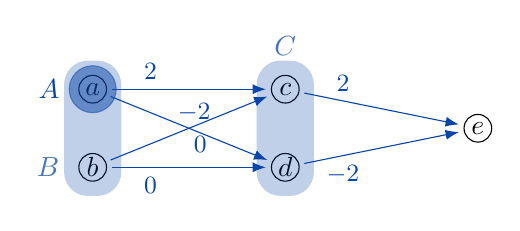
\begin{tikzpicture}[loose/.style={inner sep=.7em},edge/.style = {->,-Latex},
oval/.style={ellipse,draw}]

% nodes
\node[circle,minimum size=10pt,inner sep=0pt,outer sep=2pt,fill=white,draw](a){$a$};
\node[below=0.5 of a,circle,minimum size=10pt,inner sep=0pt,outer sep=2pt,fill=white,draw](b){$b$};

\node[right=2.2 of $(a)$,circle,minimum size=10pt,inner sep=0pt,outer sep=2pt,fill=white,draw](c){$c$};
\node[right=2.2 of $(b)$,circle,minimum size=10pt,inner sep=0pt,outer sep=2pt,fill=white,draw](d){$d$};

\node[right=2.2 of $(c)!0.5!(d)$,circle,minimum size=10pt,inner sep=0pt,outer sep=2pt,fill=white,draw](e){$e$};

% sets
\node[fill=myblue,color=myblue, opacity=0.5,oval,fit=(a),inner sep=-1pt]{};
\node[fill=myblue, opacity=0.25,rectangle,rounded corners=2ex,fit=(a) (b)]{};
\node[fill=myblue, opacity=0.25,rectangle,rounded corners=2ex,fit=(c) (d)]{};

% set labels
\node [color=myblue,opacity=1,left=0.3 of $(a)$]{$A$};
\node [color=myblue,opacity=0.75,left=0.3 of $(b)$]{$B$};
\node [color=myblue,opacity=0.75,above=0.3 of $(c)$]{$C$};

\draw[edge, color=myblue] (a) -- (c) node [near start, above] {\small{\textbf{$2$}}};
\draw[edge, color=myblue] (b) -- (c) node [near end, left=0.10] {\small{\textbf{$-2$}}};
\draw[edge, color=myblue] (a) -- (d) node [near end, left=0.15] {\small{\textbf{$0$}}};
\draw[edge, color=myblue] (b) -- (d) node [near start, below] {\small{\textbf{$0$}}};
\draw[edge, color=myblue] (c) -- (e) node [near start, above] {\small{\textbf{$2$}}};
\draw[edge, color=myblue] (d) -- (e) node [near start, below] {\small{\textbf{$-2$}}};
\end{tikzpicture}
}
\caption{\textcolor{myred}{TODO}}
\label{fig:monotonicity-counterexamples}
\end{figure}
%-------------------------------------------------------
%-------------------------------------------------------

In the terminology of \citep{kraus1990nonmonotonic}, $\Prop$ is \emph{loop-cumulative} --- it satisfies both the cumulative and loop properties above.  In fact, $\Prop$ is \emph{not} a fully monotonic closure operator, as the following fact shows.

\begin{proposition}
It is not the case that for all $S_1, S_2 \in \Set$, if $S_1 \subseteq S_2$, then $\Prop(S_1) \subseteq \Prop(S_2)$.
\end{proposition}
\begin{proof}
Consider the BFNN $\Net$ in Figure~\ref{fig:monotonicity-counterexamples}. Let $O^{(n)} \circ A^{(n)}$ be determined by a step function with threshold $0$, i.e. $O^{(n)}(A^{(n)}(x)) = 1$ iff $x > 0$.  We have $S_1 = \set{a} \subseteq \set{a, b} = S_2$, and so the hypothesis holds. But $\Prop(S_1) = \set{a, c} \not \subseteq \set{a, b} = \Prop(S_2)$. (Observe that $c$ does not get activated in $\Prop(S_2)$ because the weights cancel each other.)
\end{proof}

%OLD, we have a proof now.
%The reason for this is that a BFNN's weights $W_{ij}$ can be negative, which allows $S_2$ to inhibit the activation of new neurons that were otherwise activated by $S_1$.

%═══════════════════════════════════════════
\section{From Hebbian Learning to Logic}
%═══════════════════════════════════════════

\subsection{The Dynamics of Hebbian Learning}
%═══════════════════════════════════════════

The plan from here is to extend this logic of propagation by providing an account of Hebbian learning.  Our goal is to cast Hebbian update as a dynamic modality, so that we can explore its interactions with $\Prop$ in symbolic language.  As with $\Prop$, we start by outlining the algebraic structure of Hebbian update.

Hebb's classic learning rule \citep{hebb-organization-of-behavior-1949} states that when two adjacent neurons are simultaneously and persistently active, the connection between them strengthens.  In contrast with, e.g. backpropagation, Hebbian learning is errorless and unsupervised.  Another key difference is that Hebbian update is local --- the change in a weight $\Delta W_{ij}$ depends only on the activation of the immediately adjacent neurons.  For this reason, the Hebbian family of learning policies has traditionally been considered more biologically plausible than backpropagation.  There are many variations of Hebbian learning, but we only consider the most basic (unstable, no weight decay) form of Hebb's rule:  $\Delta W_{ij} = \eta x_i x_j$, where $\eta$ is the learning rate and $x_i, x_j$ are the outputs of adjacent neurons $i$ and $j$, respectively.

In order to incorporate Hebb's rule into our framework, we introduce a function $\Inc$ (``Hebbian update'') to strengthen those edges in a BFNN $\Net$ whose neurons are active when we feed $\Net$ a signal $S \in \Set$.  
% SAVE EXPOSITION FOR THE JOURNAL
% ALSO needs to be rephrased, technically incorrect
%We can get the output of a neuron $n$ via the following characteristic function.
% \begin{definition}
% For $S \in \Set$, let 
% $\bigchi_S : N \to \set{0, 1}$ be given by $\bigchi_S(n) = 1$ iff $n \in S$
% \end{definition}

% SAVE EXPOSITION FOR THE JOURNAL
% $\Inc$ can now be defined as follows.
\begin{definition}
\label{def:inc}
Let ${\Inc : \AllNets \times \Set \to \AllNets}$ be given by $\Inc(\langle N, E, W, A, O, \eta \rangle, S) = \langle N, E, W^\ast, A, O, \eta \rangle$, where
\[
    W_{ij}^\ast = W_{ij} + \eta \cdot \bigchi_{\Prop(S)}(i) \cdot  \bigchi_{\Prop(S)}(j)
\]
\end{definition}
Notice that we propagate $S$ before getting the active status of neurons. This is because otherwise we would never strengthen connections beyond the input layer. Now let's consider the algebraic properties of $\Inc$. We were able to formulate the algebraic properties of $\Prop$ in terms of $\Set$ containment. Similarly, we can express certain properties of $\Inc$ in terms of $\AllNets$ containment.
% Similar to our $\overrightarrow{W}$ notation, when $m_i$ is drawn from a sequence ${m_1, \ldots, m_k}$ we write $\overrightarrow{\bigchi}_S(m_i, n)$ to denote the sequence $\bigchi_S(m_1) \cdot \bigchi_S(n), \ldots, \bigchi_S(m_k) \cdot \bigchi_S(n)$.  
% SAVE EXPOSITION FOR JOURNAL VERSION
%We define the notion of \emph{subnet} ($\preceq$) as follows.

\begin{definition}
Let $\Net_1, \Net_2 \in \AllNets$ differ only in their weights.  We write
\[
    \Net_1 \preceq \Net_2
\]
to mean that for all $S \in \Set$, $\Prop_{\Net_1}(S) \subseteq \Prop_{\Net_2}(S)$.  We use $\Net_1 \cong \Net_2$ to express that $\Net_1 \preceq \Net_2$ and $\Net_2 \preceq \Net_1$.
\end{definition}

% For example, $\Inc(\Net, S)$ is a supernet of $\Net$ because strengthening weights via the $\Inc$ operation only has the potential to \emph{expand} future propagations.  
For example, consider the least upper bound $\mathcal{N}^{lub}$ of $\preceq$.  $\mathcal{N}^{lub}$ is that net whose weights have been ``maximally'' strengthened --- that is, increased to the point that every propagation $\Prop(S)$ results in all neurons graph-reachable from $S$.  By construction, $\mathcal{N}^{lub}$ is a supernet of every other net.
% To further cement this intuition, 

We have the following test to determine if $\Net_1 \preceq \Net_2$.
\begin{lemma}
\label{lemma:subnet->leq}
Suppose $\Net_1$ and $\Net_2$ are the same except for their weights, and let $S \in \Set$.  Then ${\Prop_{\Net_1}(S) \subseteq \Prop_{\Net_2}(S)}$ iff for all $n$ and all $m_1, \ldots, m_k$ such that $(m_i, n) \in E$,
\begin{equation}\tag{$\ast\ast$}
\label{eqn:weight-condition}
  \begin{gathered}
    O^{(n)}(A^{(n)}(\sum_{m_i{E}n} W_{\Net_1}(m_i, n) \cdot \bigchi_{\Prop_{\Net_1}(S)}(m_i))) = 1 \\
    \mbox{implies} \\
    O^{(n)}(A^{(n)}(\sum_{m_i{E}n} W_{\Net_2}(m_i, n) \cdot \bigchi_{\Prop_{\Net_2}(S)}(m_i))) = 1
  \end{gathered}
\end{equation}
In words: For all $S, n$, if $n$ is activated by its predecessors in $\Net_1$, then it is activated by its predecessors in $\Net_2$ as well.
\end{lemma}
\begin{proof}
($\rightarrow$) Consider the contrapositive; suppose that there are $m_1, \ldots, m_k, n$ such that $(m_i, n) \in E$ with
\[
O^{(n)}(A^{(n)}(\sum_{m_i{E}n} W_{\Net_1}(m_i, n) \cdot \bigchi_{\Prop_{\Net_1}(S)}(m_i))) = 1
\]
and yet
\[
O^{(n)}(A^{(n)}(\sum_{m_i{E}n} W_{\Net_2}(m_i, n) \cdot \bigchi_{\Prop_{\Net_2}(S)}(m_i))) = 0
\]
% Let $S = \set{m_1, \ldots, m_k}$.  
But by definition of $\Prop$, this means $n \in \Prop_{\Net_1}(S)$, but $n \not \in \Prop_{\Net_2}(S)$.  So $\Prop_{\Net_1}(S) \not \subseteq \Prop_{\Net_2}(S)$.


($\leftarrow$) We need to show that $\Prop_{\Net_1}(S) \subseteq \Prop_{\Net_2}(S)$. Let $n \in \Prop_{\Net_1}(S)$. We show $n \in \Prop_{\Net_2}(S)$ by structural induction on $\Prop_{\Net_1}(S)$:

\begin{description}
\item[Base Step:] $n \in S$. But then $n \in \Prop_{\Net_2}(S)$ by the base case of $\Prop_{\Net_2}(S)$.

\item[Inductive Step:]
We have $n \in \Prop_{\Net_1}(S)$ from the constructor case, i.e.\ because for those $m_1, \ldots, m_k$ such that $(m_i, n) \in E$,
\[
O^{(n)}(A^{(n)}(\sum_{m_i{E}n} W_{\Net_1}(m_i, n) \cdot \bigchi_{\Prop_{\Net_1}(S)}(m_i))) = 1
\]
By assumption, for these $n$ and predecessors $m_1, \ldots, m_k$ in particular,
\[
O^{(n)}(A^{(n)}(\sum_{m_i{E}n} W_{\Net_2}(m_i, n) \cdot \bigchi_{\Prop_{\Net_2}(S)}(m_i))) = 1
\]
Notice that our hypothesis is so strong that there is no need to apply our inductive hypothesis. We immediately get, by definition of $\Prop$, $n \in \Prop_{\Net_2}(S)$. \qedhere
\end{description}
\end{proof}

\begin{corollary}
\label{corollary:subnet->weights}
Let $\Net_1, \Net_2$ be the same except for their weights.  Then $\Net_1 \preceq \Net_2$ iff for all $n \in N$ and for those $m_1, \ldots, m_k \in N$ such that $(m_i, n) \in E$, (\ref{eqn:weight-condition}) holds.
\end{corollary}
\begin{proof}
This follows straightforwardly from the previous lemma:
\[
\begin{array}{lcll}
    \Net_1 \preceq \Net_2 & \mbox{iff} & \mbox{for all } S, \Prop_{\Net_1}(S) \subseteq \Prop_{\Net_2}(S) & (\mbox{By defn of } \preceq) \\
    & \mbox{iff} & \mbox{(\ref{eqn:weight-condition}) holds for all } n \mbox{ and its predecessors }m_1, \ldots, m_k & (\mbox{By Lemma~\ref{lemma:subnet->leq}})
\end{array} \qedhere
\]
\end{proof}
This test is a convenient way to show $\Net_1 \preceq \Net_2$: prove that for all $n$, if $n$ activates in $\Net_1$ then $n$ activates in $\Net_2$. But the test is not always applicable --- often we still need to do a full proof by induction and leverage the inductive hypothesis to prove net containment properties. But the proof is still worth understanding, since it serves as an example for how to do these (somewhat nasty) inductive proofs.

We are now ready to state and prove the following algebraic characterization of $\Inc$. Note that $\Prop(S)$ abbreviates $\Prop_\Net(S)$, the propagation in the net before update.

\begin{theorem}
For all $\Net, \Net_1, \Net_2 \in \AllNets$ and $A, B, B_1, \ldots, B_k \in \Set$, $\Inc$ satisfies
\begin{description}
    \item[(Monotonicity in $\Net$)] if ${\Net_1 \preceq \Net_2}$
    then ${\Inc(\Net_1, A) \preceq \Inc(\Net_2, A)}$

    \item[(Absorption)]
    $\Inc(\Net, \Prop(A)) \cong \Inc(\Net, A)$
    
    \item[(Local)]
    $\Prop_{\Inc(\Net, A)}(B) \subseteq \Prop(A) \cup \Prop(B)$
    
    \item[(Cumulative)] If ${\Prop(B_1) \subseteq \Prop(B_2)}$ and ${\Prop(B_2) \subseteq \Prop_{\Inc(\Net, A)}(B_1)}$,\\
    then $\Prop_{\Inc(\Net, A)}(B_1) = \Prop_{\Inc(\Net, A)}(B_2)$
    
    \item[(Loop)] If ${\Prop(B_1) \subseteq \Prop_{\Inc(\Net, A)}(B_0)}$,
    $\ldots, {\Prop(B_n) \subseteq \Prop_{\Inc(\Net, A)}(B_{n-1})}$,\\
    and 
    ${\Prop(B_0) \subseteq \Prop_{\Inc(\Net, A)}(B_n)}$,
    then ${\Prop_{\Inc(\Net, A)}(B_i) = \Prop_{\Inc(\Net, A)}(B_j)}$
    for all $i, j \in \set{0, \ldots, n}$
\end{description}
\label{thm:inc-props}
\end{theorem}
\begin{proof} Unfortunately, we are not able to use Lemma~\ref{lemma:subnet->leq}, so we resort to doing full proofs by induction on $\Prop$.
\begin{description}
    %═══════════════════════════════════════════%%%%%%%%%%
    \item[(Monotonicity in $\Net$)] 
    Suppose $\Net_1 \preceq \Net_2$, i.e.\ for all $B$, $\Prop_{\Net_1}(B) \subseteq \Prop_{\Net_2}(B)$. Now let $A, B \in \Set$. We want to show that $\Inc(\Net_1, A) \preceq \Inc(\Net_2, A)$; in other words, for all $A, B$,
    \[
        \Prop_{\Inc(\Net_1, A)}(B) \subseteq \Prop_{\Inc(\Net_2, A)}(B)
    \]
    Let $n \in \Prop_{\Inc(\Net_1, A)}(B)$, and proceed by induction on the structure of this $\Prop$.
    \begin{description}
        \item[Base Step:] $n \in B$. So $n \in \Prop_{\Inc(\Net_2, A)}(B)$ by the base case of $\Prop$.
        \item[Inductive Step:] We have $n \in \Prop_{\Inc(\Net_1, A)}(B)$ from the constructor case, i.e. because for those $m_1, \ldots, m_k$ such that $(m_i, n) \in E$,
        \[
            O^{(n)}(A^{(n)}(\sum_{m_i{E}n} W_{\Inc(\Net_1, A)}(m_i, n) \cdot \bigchi_{\Prop_{\Inc(\Net_1, A)}(B)}(m_i))) = 1
        \]
        \textbf{TODO}
    \end{description}
    

    %═══════════════════════════════════════════%%%%%%%%%%
    \item[(Absorption)] 
    To prove $\Inc(\Net, \Prop(A)) \cong \Inc(\Net, A)$, we need to show that for all sets $A, B$,
    \[
        \Prop_{\Inc(\Net, \Prop(A))}(B) = \Prop_{\Inc(\Net, A)}(B)
    \]
    For the $(\supseteq)$ direction, let $n \in \Prop_{\Inc(\Net, \Prop(A))}(B)$. We proceed by induction on this $\Prop$.
    \begin{description}
        \item[Base Step:] $n \in B$, and so $n \in \Prop_{\Inc(\Net, A)}(B)$ by the base case of $\Prop$.
        \item[Inductive Step:] Let $m_1, \ldots, m_k$ be the predecessors of $n$. We have
        \[
            O^{(n)}(A^{(n)}(\sum_{m_i{E}n} W_{\Inc(\Net, \Prop(A))}(m_i, n) \cdot \bigchi_{\Prop_{\Inc(\Net, \Prop(A))}(B)}(m_i))) = 1
        \]
        First, by inductive hypothesis, each $m_i \in \Prop_{\Inc(\Net, \Prop(A))}(B)$ iff $m_i \in \Prop_{\Inc(\Net, A)}(B)$, and so 
        \[
            O^{(n)}(A^{(n)}(\sum_{m_i{E}n} W_{\Inc(\Net, \Prop(A))}(m_i, n) \cdot \bigchi_{\Prop_{\Inc(\Net, A)}(B)}(m_i))) = 1
        \]
        From here, we expand the weights in the updated net $\Inc(\Net, \Prop(A))$:
        \[
            O^{(n)}(A^{(n)}(\sum_{m_i{E}n} 
            \left( W_\Net(m_i, n) \cdot \bigchi_{\Prop(\Prop(A))}(m_i) \cdot \bigchi_{\Prop(\Prop(A))}(n) \right) 
            \cdot \bigchi_{\Prop_{\Inc(\Net, A)}(B)}(m_i))) = 1
        \]
        By idempotence of $\Prop$, we can collapse each $\Prop(\Prop(A)) = \Prop(A)$.
        \[
            O^{(n)}(A^{(n)}(\sum_{m_i{E}n} 
            (W_\Net(m_i, n) \cdot \bigchi_{\Prop(A)}(m_i) \cdot \bigchi_{\Prop(A)}(n)) 
            \cdot \bigchi_{\Prop_{\Inc(\Net, A)}(B)}(m_i))) = 1
        \]
        But these is exactly the weights for $\Inc(\Net, A)$, and so
        \[
            O^{(n)}(A^{(n)}(\sum_{m_i{E}n} W_{\Inc(\Net, A)}(m_i, n) \cdot \bigchi_{\Prop_{\Inc(\Net, A)}(B)}(m_i))) = 1
        \]
        We conclude that $n \in \Prop_{\Inc(\Net, A)}(B)$, by the constructor of $\Prop$.
    \end{description}
    As for the $(\supseteq)$ direction, both the base step and inductive step hold similarly (this time, expanding the nested $\Prop$ using idempotence in reverse).
    
    %═══════════════════════════════════════════%%%%%%%%%%
    \item[(Local)]
    Rather than showing $\Prop_{\Inc(\Net, A)}(B) \subseteq \Prop(A) \cup \Prop(B)$ directly, we instead prove a stronger claim:
    \begin{equation}\tag{$\ast\ast\ast$}
    \label{local-lemma}
        \Prop_{\Inc(\Net, A)}(B) - \Prop(A) = \Prop(B) - \Prop(A)
    \end{equation}
    First, let's explain why this is sufficient. Suppose $n \in \Prop_{\Inc(\Net, A)}(B)$. There are two cases:
    \begin{itemize}
        \item $n \in \Prop(A)$. So clearly $n \in \Prop(A) \cup \Prop(B)$.
        \item $n \not \in \Prop(A)$. So $n \in \Prop_{\Inc(\Net, A)}(B) - \Prop(A)$. By (\ref{local-lemma}), this means $n \in \Prop(B) - \Prop(A)$. But then $n \in \Prop(B)$, so $n\in \Prop(A) \cup \Prop(B)$.
    \end{itemize}
    This means that (\ref{local-lemma}) implies the Local property. We have left to prove (\ref{local-lemma}). For the $(\subseteq)$ direction, suppose $n \in \Prop_{\Inc(\Net, A)}(B) - \Prop(A)$, and proceed by structural induction on $\Prop_{\Inc(\Net, A)}(B)$.
    \begin{description}
        \item[Base Step:] $n \in B$. By the base case of $\Prop$, $n \in \Prop(B)$. So $n \in \Prop(B) - \Prop(A)$.

        \item[Inductive Step:] Let $m_1, \ldots, m_k$ be the predecessors of $n$. We have
        \[
            O^{(n)}(A^{(n)}(\sum_{m_i{E}n} W_{\Inc(\Net, A)}(m_i, n) \cdot \bigchi_{\Prop_{\Inc(\Net, A)}(B)}(m_i))) = 1
        \]
        
    \end{description}

    
    %═══════════════════════════════════════════%%%%%%%%%%
    \item[(Cumulative \& Loop)] Finally, the Cumulative and Loop properties for $\Inc$ follow from the Cumulative and Loop properties for $\Prop$ in Theorem~\ref{thm:prop-props} by substituting (for each $i \in \set{0, \ldots, n}$)
    \[
    \begin{array}{lcl}
    
    \Net & \rightsquigarrow & \Inc(\Net, A)\\
    B_i & \rightsquigarrow & \Prop_\Net(B_i)
    
    \end{array}
    \]
\end{description}
\end{proof}

\begin{proposition}
$\Inc$ is not monotonic in $S$.
\end{proposition}  
\begin{proof}
\textbf{\textcolor{myred}{FILL IN}}
\end{proof}

\subsection{Syntax and Semantics}
%═══════════════════════════════════════════

We can now introduce the logic of Hebbian learning.  Let $p, q, \ldots$ be finitely many propositional variables.  These represent fixed, `ontic' states, i.e. established choices of neurons that correspond to features in the external world.  For example, $p$ might be the set of neurons that encapsulates the color \emph{pink}.  We presume that we already agree on these states, although we acknowledge that this is a major unresolved empirical issue.  As for more complex formulas:

\begin{definition}  Formulas of our language $\lang$ are given by
\[
\varphi \Coloneqq p \mid \neg \varphi \mid \varphi \land \varphi \mid \varphi \Rightarrow \varphi \mid \Typ \varphi \mid [\varphi^+] \varphi
\]
where $p$ is any propositional variable.  We define $\top$, $\bot$, $\lor$, $\to$, $\leftrightarrow$, $\Leftrightarrow$, and the dual modalities $\langle \Typ \rangle, \langle \varphi^+ \rangle$ in the usual way.
\end{definition}

The modalities $\Typ$ and $[\varphi^+]$ reflect our two operations $\Prop$ and $\Inc$, respectively.  We intend for $\Typ \varphi$ to denote ``the propagation of signal $\varphi$,'' and for $[\varphi^+] \psi$ to denote ``after performing Hebbian update on $\varphi$, evaluate $\psi$.''  We import ${\varphi \Rightarrow \psi}$ from \citep{leitgeb2001nonmonotonic}, read ``the propagation of signal $\varphi$ contains $\psi$''.  Note that ${\varphi \Rightarrow \psi}$ is redundant (equivalent to $\Typ \varphi \to \psi$ using the semantics below), though we keep it in our syntax because it conveniently expresses ``the net \emph{classifies} $\varphi$ as $\psi$'' (if $\varphi$ is interpreted as an input and $\psi$ as a classification).

Our formulas also have more classical alternative readings, divorced from the dynamics of neural networks.  Following \citep{leitgeb2001nonmonotonic}, we will define $\varphi \Rightarrow \psi$ such that it has the conditional reading ``typically $\varphi$ are $\psi$'' (where $\varphi$ and $\psi$ are read as generics, e.g. ``typically birds fly'').  This gives us a natural preferential reading for $\Typ \varphi$ as ``typically $\varphi$'' or ``the typical $\varphi$.''\footnote{Our notation takes inspiration from \citep{giordano2021}, which formalizes the dynamics of a net via a concept constructor $\Typ$ in the description logic $\mathcal{ALC}$.  Note the subtle difference between their typicality inclusions $\Typ(\varphi) \sqsubseteq \psi$ and our $\Typ \varphi \to \psi$: Ours flips the direction of containment.} 
Finally, Hebbian learning $[\varphi^+] \psi$ has a dual reading as \emph{preference upgrade}  \citep{van2007prefupgrade}.  As mentioned in the Related Work section, we leave the question concerning how $[\varphi^+]$ can be viewed classically as updating a preference relation to future work.

A model of our logic is just a BFNN $\Net$ equipped with an interpretation function $\semantics{\cdot} : \lang \to \Set_\Net$.

\begin{definition}
Let $\Net \in \AllNets$.  Our semantics are defined recursively as follows:
\begin{equation*}
\boxed{
\begin{array}{lcl}
\semantics{p} & & \in \Set \mbox{ is fixed, nonempty} \\
\semantics{\top} & = & \emptyset\\
\semantics{\neg \varphi} & = & \overline{\semantics{\varphi}}\\
\semantics{\varphi \land \psi} & = & \semantics{\varphi} \cup \semantics{\psi}\\
\semantics{\varphi \Rightarrow \psi} & = & \semantics{\Typ \varphi \to \psi}\\
\semantics{\Typ \varphi} & = & \Prop(\semantics{\varphi}) \\
\semantics{[\varphi^+] \psi} & = & \semantics{\psi}_{\Inc(\Net, \semantics{\varphi})} \\
\end{array}
}
\end{equation*}
\end{definition}

Notice that these semantics are ``flipped'' in the sense that $\land$ is interpreted as union (instead of intersection), and consequently $\to$ is interpreted as superset (instead of subset).  This choice may seem odd, but it  reflects the intuition that neurons act as ``elementary-feature-detectors'' \citep{leitgeb2001nonmonotonic}.  
% possible thing to remove:
For example, say $\semantics{\varphi}$ represents those neurons that are \textit{necessary} for detecting an apple, and $\semantics{\psi}$ represents those neurons that are \textit{necessary} for detecting the color red. 
% add 'for instance,'
If the net observes a red apple ($\varphi \land \psi$), both the neurons detecting red-features $\semantics{\varphi}$ and the neurons detecting apple-features $\semantics{\psi}$ necessarily activate, i.e. $\semantics{\varphi} \cup \semantics{\psi}$ activates.  As for implication, ``every apple is red'' (${\varphi \to \psi}$) holds for a net iff whenever the neurons detecting apple-features $\semantics{\varphi}$ necessarily activate, so do the neurons detecting red-features $\semantics{\psi}$.  But this is only true if ${\semantics{\varphi} \supseteq \semantics{\psi}}$.  This justifies us reading propositional connectives classically, despite the backwards flavor of the semantics.


Our interpretation of formulas is completely algebraic, in the sense that formulas denote sets rather than truth-values.  But we can consider formulas to have truth-values as follows.

\begin{definition}
$\Net \models \varphi$ iff $\semantics{\varphi}_\Net = \emptyset$.
\end{definition}

This choice also appears to be strange at its surface.  But it is a natural one in light of the fact that we defined $\semantics{\top} \coloneqq \emptyset$.  For example, consider implication: $\Net \models \varphi \to \psi$ holds iff $\semantics{\varphi \to \psi} = \emptyset = \semantics{\top}$, which holds iff $\semantics{\varphi} \supseteq \semantics{\psi}$ by our semantics.

A curious consequence is that if $\Net \models \varphi$ and $\varphi$ cannot be written to contain an implication $\to$, then $\varphi$ must be a tautology.  But we do not consider this troubling, since it only makes sense to consider a neural network's judgment of $\varphi$ when given a state $\semantics{\psi}$ the net is in.

\begin{figure}[ht!]
\begin{equation*}
\boxed{
\begin{array}{ll}
    %----------------------------------
    % Basic Axioms and Inference Rules
    \textbf{Basic Axioms and Inference Rules} &
    \Typ \textbf{ Axioms} \\
    
    \begin{array}{ll}
         \axiom{(PC)} & \mbox{All propositional tautologies}\\
    
        \axiom{(MP)} & \frac{\varphi \quad \varphi \to \psi}{\psi} \\
        
        (\axiom{Nec}_\Typ) & \frac{\varphi}{\Typ \varphi}\\
        
        (\axiom{Nec}_+) & \frac{\psi}{[\varphi^+] \psi}\\
    \end{array} &
    
    \begin{array}{ll}
        (\axiom{Loop}) & 
        (\Typ \varphi_0 \to \varphi_1)
        \land \cdots \land 
        (\Typ \varphi_k \to \varphi_0) 
        \\
        & \quad \to (\Typ \varphi_0 \leftrightarrow \Typ \varphi_k) \\
         
        \axiom{(Dual)} & \langle \Typ \rangle \varphi \leftrightarrow \neg \Typ \neg \varphi\\
    
        \axiom{(T)} & \Typ \varphi \to \varphi\\
        
        \axiom{(4)} & \Typ \varphi \to \Typ \Typ \varphi\\
    \end{array}
    
    \\ \\
    %----------------------------------
    % Reduction Axioms
    \textbf{Reduction Axioms} & \textbf{Interaction Axioms}\\
    
    \begin{array}{ll}
         (\axiom{R}_p) & [\varphi^+] p \leftrightarrow p \\
    
        (\axiom{R}_\neg) & [\varphi^+] \neg \psi \leftrightarrow \neg [\varphi^+] \psi \\
        
        (\axiom{R}_\land) & [\varphi^+] (\psi \land \rho) \leftrightarrow ([\varphi^+] \psi \land [\varphi^+] \rho)\\
    \end{array}
    &
    \begin{array}{ll}
        (\axiom{Nest}_\Typ) & [\Typ \varphi^+] \psi \leftrightarrow [\varphi^+] \psi \\
    
         % Agent prefers the result of update in advance
        % "No Disappointment"
        \axiom{(NS)} & [\varphi^+] \Typ \psi \to \Typ [\varphi^+] \psi\\
        
        % "Preference Persistence"
        % (one of the four major effects under the umbrella of "confirmation bias"
        \axiom{(TP)} & \Typ [\varphi^+] \psi \land \Typ \varphi \to [\varphi^+] \Typ \psi\\
    \end{array}
    \\
\end{array}
}
\end{equation*}
\caption{A list of sound rules and axioms of the logic of Hebbian learning.  We leave the question of completeness to future work.}
\label{fig:proof-system}
\end{figure}

\subsection{Inference and Axioms}
%═══════════════════════════════════════════

The proof system for our logic is as follows.  We have $\proves \varphi$ iff either $\varphi$ is an axiom, or $\varphi$ follows from previously obtained formulas by one of the inference rules.  If $\Gamma \subseteq \lang$ is a set of formulas, we consider $\Gamma \proves \varphi$ to hold whenever there exist finitely many $\psi_1, \ldots, \psi_k \in \Gamma$ such that $\proves \psi_1 \land \ldots \land \psi_k \to \varphi$.

We list the axioms and inference rules for our logic in Figure~\ref{fig:proof-system}.  Our main result is the soundness of these axioms and rules --- we do not claim that this list forms a complete axiomatization (we revisit the question of completeness in the Conclusion).

The static base of our logic is the modal logic characterized by $\Typ$.  If we translate $\varphi \Rightarrow \psi$ via $\Typ \varphi \to \psi$ as before, we see that this modal logic contains the conditional logic \textbf{CL} (loop-cumulative).  As a modality, $\Typ$ is neither normal, regular, nor monotonic, but it is classical.  Note for instance that the normal modal property \axiom{(K)} (expressed in terms of $\Typ$) is equivalent to
\[
\axiom{(K)} \quad \Typ (\varphi \land \psi) \leftrightarrow (\Typ \varphi \land \Typ \psi)
\]
neither direction of which is sound in our logic.  Instead, we have the $\axiom{(Loop)}$ axiom expressing the loop-cumulativity of $\Prop$.  In fact, $\axiom{(Loop)}$ is all that is needed for this weakening of monotonicity --- note that we have dropped cumulativity $(\axiom{C}_\Rightarrow)$, as well as $(\axiom{Loop}_+)$ and $(\axiom{C}_+)$ for $[\varphi^+]$, since they all follow from the present axioms (compare against \citep{kisby2022logic}).

Since Hebbian update only affects the propagation of states, we have reduction axioms $(\axiom{R}_p), (\axiom{R}_\neg), (\axiom{R}_\land)$, as well as the axiom $(\axiom{Nest}_\Typ)$ for terms that nest $\Typ$ within $[\varphi^+]$.

In lieu of a full reduction for $[\varphi^+] \Typ \psi$, we instead have the weaker axioms $\axiom{(NS)}$ and $\axiom{(TP)}$.  These two axioms capture key cognitive biases of a Hebbian agent.  Consider the axiom $\axiom{(TP)}$, i.e. (Typicality Preservation)
\[
\axiom{(TP)} \quad \Typ [\varphi^+] \psi \land \Typ \varphi \to [\varphi^+] \Typ \psi
\]
This says that if our agent expects $\psi$ is normally true after learning $\varphi$, but she also happens to expect $\varphi$, then after learning $\varphi$ the typicality of $\psi$ will be preserved.  This is a peculiar kind of cognitive bias whereby a Hebbian agent maintains her prior attitudes when presented with news she already expects.

The axiom $\axiom{(NS)}$, i.e. (No Surprises)
\[
\axiom{(NS)} \quad [\varphi^+] \Typ \psi \to \Typ [\varphi^+] \psi
\]
says that if after learning $\varphi$, our agent thinks normally $\psi$, then she would have expected $\psi$ to be true after learning $\varphi$ in the first place.  Loosely: She will never be surprised.


% COMMENT TO MAKE ON THE JOURNAL VERSION:
% Notes: we give reductions in terms of \neg and \land (which covers implication, top, and bot), primarily because of the lemma that makes nested implications useless (so we have to rephrase (K) for [\varphi^+], for instance)

% COMMENT TO MAKE ON THE JOURNAL VERSION:
% To check the validity of each of these axioms and rules, we make use of the following technical fact.  Notice that it follows that antecedents in right-associated implications get absorbed, e.g. $\varphi \to (\psi \to \rho)$ reduces to $\psi \to \rho$.
% \begin{lemma}
% Suppose $S \ne N$.  Then $\Net, S \models \varphi \to \psi$ iff $\Net, \semantics{\varphi}_\Net \models \psi$ (iff $\semantics{\psi}_\Net \subseteq \semantics{\varphi}_\Net$).
% \end{lemma}

Soundness of these axioms is largely a matter of matching each axiom with its corresponding property of $\Inc$.

\begin{theorem}
The rules and axioms above are sound, i.e. hold for all $\Net \in \AllNets$.
\end{theorem}
\begin{proof}
\textbf{\textcolor{myred}{FILL IN}}
\end{proof}

%═══════════════════════════════════════════
\section{Applying the Logic: A Concrete Example}
%═══════════════════════════════════════════
\label{sec:concrete}

\begin{figure}
\centering{
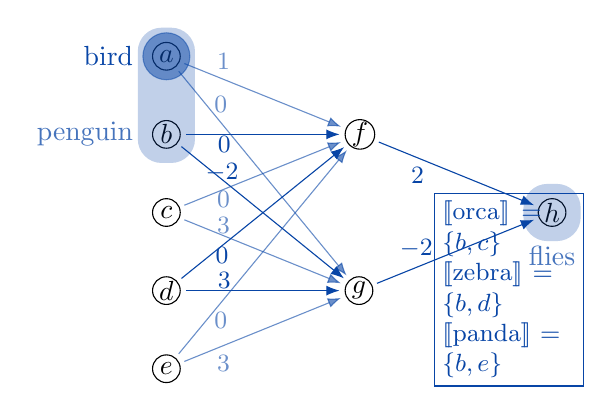
\begin{tikzpicture}[loose/.style={inner sep=.7em},edge/.style = {->,-Latex},
oval/.style={ellipse,draw}]

% nodes
\node[circle,minimum size=10pt,inner sep=0pt,outer sep=2pt,fill=white,draw](a){$a$};
\node[below=0.5 of a,circle,minimum size=10pt,inner sep=0pt,outer sep=2pt,fill=white,draw](b){$b$};
\node[below=0.5 of b,circle,minimum size=10pt,inner sep=0pt,outer sep=2pt,fill=white,draw](c){$c$};
\node[below=0.5 of c,circle,minimum size=10pt,inner sep=0pt,outer sep=2pt,fill=white,draw](d){$d$};
\node[below=0.5 of d,circle,minimum size=10pt,inner sep=0pt,outer sep=2pt,fill=white,draw](e){$e$};

\node[right=2.2 of $(a)!0.5!(c)$,circle,minimum size=10pt,inner sep=0pt,outer sep=2pt,fill=white,draw](f){$f$};
\node[right=2.2 of $(c)!0.5!(e)$,circle,minimum size=10pt,inner sep=0pt,outer sep=2pt,fill=white,draw](g){$g$};

\node[right=2.2 of $(f)!0.5!(g)$,circle,minimum size=10pt,inner sep=0pt,outer sep=2pt,fill=white,draw](h){$h$};

% Hidden nodes
\node (bpivot) [left=0.3 of b] {\phantom{p}};
\node (dpivot) [left=0.3 of d] {\phantom{p}};
\node (bpivot2) [right=0.3 of b] {\phantom{p}};
\node (epivot) [right=0.3 of e] {\phantom{p}};

% sets
\node[fill=myblue,color=myblue, opacity=0.5,oval,fit=(a),inner sep=-1pt]{};
\node[fill=myblue, opacity=0.25,rectangle,rounded corners=2ex,fit=(a) (b)]{};
\node[fill=myblue, opacity=0.25,rectangle,rounded corners=2ex,fit=(h)]{};


% set labels
\node [color=myblue,opacity=1,left=0.3 of $(a)$]{bird};
\node [color=myblue,opacity=0.75,left=0.3 of $(b)$]{penguin};
\node [color=myblue,opacity=0.75,below=0.3 of $(h)$]{flies};

\draw[edge, color=myblue, opacity=0.6] (a) -- (f) node [near start, above] {\small{\textbf{$1$}}};
\draw[edge, color=myblue, opacity=0.6] (a) -- (g) node [near start, above] {\small{\textbf{$0$}}};
\draw[edge, color=myblue] (b) -- (f) node [below=-0.1, near start] {\small{\textbf{$0$}}};
\draw[edge, color=myblue] (b) -- (g) node [near start, above=-0.15] {\small{\textbf{$-2$}}};
\draw[edge, color=myblue, opacity=0.6] (c) -- (f) node [near start, below=-0.1] {\small{\textbf{$0$}}};
\draw[edge, color=myblue, opacity=0.6] (c) -- (g) node [near start, above=-0.1] {\small{\textbf{$3$}}};
\draw[edge, color=myblue] (d) -- (f) node [near start, below=-0.1] {\small{\textbf{$0$}}};
\draw[edge, color=myblue] (d) -- (g) node [near start, above=-0.1] {\small{\textbf{$3$}}};
\draw[edge, color=myblue, opacity=0.6] (e) -- (f) node [near start, below] {\small{\textbf{$0$}}};
\draw[edge, color=myblue, opacity=0.6] (e) -- (g) node [near start, below] {\small{\textbf{$3$}}};
\draw[edge, color=myblue] (f) -- (h) node [near start, below] {\small{\textbf{$2$}}};
\draw[edge, color=myblue] (g) -- (h) node [near start, above] {\small{\textbf{$-2$}}};

% KEY
\node[draw, color=myblue, text width=0.14\linewidth,inner sep=1mm,align=left,
      above left] at (current bounding box.south east)
    {\small $\semantics{\textup{orca}} = \set{b, c}$\\
    $\semantics{\textup{zebra}} = \set{b, d}$\\
    $\semantics{\textup{panda}} = \set{b, e}$\\};

\end{tikzpicture}
}
\caption{A BFNN $\Net$, equipped with the ReLU activation function, $T = 1$, and $\eta = 1$.  After observing the dataset $\langle \textrm{orca}, \textrm{zebra}, \textrm{panda} \rangle$, $\Net$ learns that penguins do not fly, while preserving the fact that birds typically fly. \textcolor{myred}{TODO}}
\label{fig:full-example}
\end{figure}

We now demonstrate our neuro-symbolic interface by way of an example neural network in a machine learning context.  The task: Given an image of an animal, classify it as flying or non-flying.  Suppose we have the partially pre-trained BFNN $\Net$ in  Figure~\ref{fig:full-example}.  

For simplification's sake, let's suppose that our animal images can be reduced to $5$-dimensional vectors in order to be fed into the input layer of $\Net$.  Say:
\[
\begin{array}{llcll}
\textrm{penguin} & \langle 1 1 0 0 0 \rangle & \quad & 
\textrm{orca} & \langle 0 1 1 0 0 \rangle \\
\textrm{zebra} & \langle 0 1 0 1 0 \rangle & \quad & 
\textrm{panda} & \langle 0 1 0 0 1 \rangle \\
\end{array}
\]
In addition, suppose an image activates the first node if and only if it depicts a bird.

We can identify each animal with the set of nodes it activates in the input layer.  This gives us the sets shown in Figure~\ref{fig:full-example}.  We can also identify the class of things that fly with the output node, i.e. $\semantics{\textup{flies}} = \set{h}$.  In principle we can identify propositions with sets containing hidden nodes as well, although in practice the meaning of hidden nodes is often unclear.

With this interpretation in mind, we see that $\Net \models \textrm{bird} \Rightarrow \textrm{flies}$, but also $\Net \models \textrm{penguin} \Rightarrow \textrm{flies}$ (which is incorrect).  Our hope is that $\Net$ corrects this mistake via Hebbian learning.

Say we expose $\Net$ to non-flying animals that share the black-and-white color of penguins, e.g. we train $\Net$ on the dataset $\langle \textrm{orca}, \textrm{zebra}, \textrm{panda} \rangle$.  The propagations of each instance will increase $W_{bg}$.  Once we have given $\Net$ the entire dataset ($W_{bg} = 1$), $\Prop(\semantics{\textup{penguin}})$ will contain $g$, which will cancel the signal given by ${f \to h}$.  Our logic successfully models this behavior:
\[
\begin{array}{l}
\Net \models [\textrm{orca}^+] [\textrm{zebra}^+] [\textrm{panda}^+] (\textrm{bird} \Rightarrow \textrm{flies}) \textrm{, yet}\\
\Net \not \models [\textrm{orca}^+] [\textrm{zebra}^+] [\textrm{panda}^+] (\textrm{penguin} \Rightarrow \textrm{flies})
\end{array}
\]
i.e. $\Net$ learns that penguins do not fly while preserving the fact that birds typically fly. 

% UPDATE: We actually give a counterexample to monotonicity in the right spot.
%---------------------------------------
% As it happens, if we modify $\Net$ such that $W_{bg} = 0$ then this serves as a counterexample to monotonicity in $S$ (see the discussion following Theorem~\ref{thm:inc-props}).  In particular, we have $\Net \models \Typ(\textrm{penguin}) \to \textrm{flies}$, yet $\Net \not \models [\textrm{orca}^+] \Typ(\textrm{penguin}) \to [\textrm{orca}^+] \textrm{flies}$. 

%═══════════════════════════════════════════
\section{Conclusion and Future Work}
%═══════════════════════════════════════════

In this paper, we gave sound axioms and rules characterizing the logic of Hebbian learning.  This logic interfaces the neuro-symbolic divide by characterizing conditionals $\Rightarrow$ and modalities $\Typ$, $[\varphi^+]$ in terms of the propagation and Hebbian update of signals in a neural network.  The upshot of all this is that this logic describes a neuro-symbolic agent that learns associatively and also reasons about what it has learned.

We leave open the question of whether the axioms and rules we list are complete.  But we take this opportunity to stress the importance of having strong completeness for logics of this kind.  Strong completeness for a \emph{static} neural semantics provides a bridge across which we can extract a set of rules $\Gamma$ from an interpreted network, and also build an interpreted neural network implementing $\Gamma$.  But once the neural network updates, we lose the interpretations of neurons that allow for these translations.  If we had strong completeness for the \emph{dynamic} logic, we could fully track the interpretations while the net learns and preserve this neuro-symbolic correspondence.

Beyond the logic of Hebbian learning, we believe that this framework will be a fruitful way to explore the neuro-symbolic interface for a variety of neural networks and learning policies.  Exciting future directions include:
\begin{enumerate}[itemsep=-1pt, topsep=2pt]
    \item Mapping more expressive syntax to neural activity
    \item Generalizing to a broader class of neural networks
    \item Generalizing to a broader class of activation functions
    \item Characterizing other learning policies in logical terms
\end{enumerate}
The holy grail of this line of work is to completely axiomatize the (1) first-order logic of (2) nonbinary (fuzzy-valued) neural networks with (3) more varied (e.g. ReLU and GELU) activation functions that (4) learn via backpropagation.

%═══════════════════════════════════════════
\section{Acknowledgements}
%═══════════════════════════════════════════
We thank the anonymous reviewers for their careful reviews and helpful comments.  C.~Kisby was supported in part by the US Department of Defense [Contract No. W52P1J2093009].

%═══════════════════════════════════════════
\section{Corrections to the FLAIRS Paper}
%═══════════════════════════════════════════
The original FLAIRS paper~\citep{kisby2022logic} contained an error, starting with the definition of propagation (Definition~\ref{def:propagation}) and affecting the results of Lemma 2, Corollary 1, Theorem 3, and Theorem 4. We only noticed the error after trying to formally verify some of these results in Lean. See our follow-up paper \citep{kisby2024hebbian}, where the major results have been checked in Lean.

In this arXiv version, we have presented corrected definitions and results. In this section we will state which statements in the FLAIRS paper were false, and explain how they have been corrected.

In the FLAIRS paper, propagation was defined as follows: 
\begin{restatedef}{3}
    Let $\Prop : \Set \to \Set$ be defined recursively as follows:  $n \in \Prop(S)$ iff either
    \begin{description}
        \item[(Base Case)] $n \in S$, or
        \item[(Constructor)] For those $m_1, \ldots, m_k \in \Prop(S)$ such that $(m_i, n) \in E$ we have
        \[
        O^{(n)}(A^{(n)}(\overrightarrow{W}(m_i, n))) = 1
        \]
    \end{description}
\end{restatedef}
The issue here is surprisingly subtle: We only apply the activation function to the weights of those predecessors that were already active in the previous step ($m_1, \ldots, m_k \in \Prop(S)$). This means that the vector $\overrightarrow{W}(m_i, n)$ doesn't comply with the arity that $A^{(n)}$ is expecting; since the arity of $A^{(n)}$ is the indegree of $n$, we must give $A^{(n)}$ the vector of weights over \emph{all} predecessors. But a more serious problem is that this tricks us into mistakenly ignoring those predecessors which were \emph{not} already active.

In machine learning work, the standard way of doing this is to feed the activation function a weighted sum of all predecessor activations. This simple fix resolves the issue. So in this draft we instead write:
\begin{restatedef}{3}
    Let $\Prop : \Set \to \Set$ be defined recursively as follows:  $n \in \Prop(S)$ iff either
    \begin{description}
        \item[(Base Case)] $n \in S$, or
        \item[(Constructor)] For those $m_1, \ldots, m_k$ such that $m_i{E}n$ we have
        \[
        O^{(n)}(A^{(n)}(\sum_{m_i{E}n} W(m_i, n) \cdot \bigchi_{\Prop(S)}(m_i))) = 1
        \]
    \end{description}
\end{restatedef}
This inner sum term reflects the weighted sum of predecessor activations, and $\bigchi_{\Prop(S)}(m_i)$ tells us whether each $m_i$ is already active (in $\Prop(S)$).

% \hline %% TODO

\begin{restatelemma}{2}
    Suppose $\Net_1$ and $\Net_2$ are the same except for their weights, and let $S \in \Set$.  Then ${\Prop_{\Net_1}(S) \subseteq \Prop_{\Net_2}(S)}$ iff for all $n \in \Prop_{\Net_1}(S)$ and for those $m_1, \ldots, m_k \in \Prop_{\Net_1}(S)$ such that $(m_i, n) \in E$,
    \begin{equation}\tag{$\ast\ast$}
      \begin{gathered}
        O^{(n)}(A^{(n)}(\overrightarrow{W}_{\Net_1}(m_i, n))) = 1 \\
        \mbox{implies} \\
        O^{(n)}(A^{(n)}(\overrightarrow{W}_{\Net_2}(m_i, n))) = 1
      \end{gathered}
    \end{equation}
\end{restatelemma}

\begin{restatecorollary}{1}
    Let $\Net_1, \Net_2$ be the same except for their weights.  Then $\Net_1 \preceq \Net_2$ iff for all $n \in N$ and for those $m_1, \ldots, m_k \in N$ such that $(m_i, n) \in E$, (\ref{eqn:weight-condition}) holds.
\end{restatecorollary}

\begin{restatetheorem}{3}
    For all $\Net, \Net_1, \Net_2 \in \AllNets$ and $S, S_1, S_2 \in \Set$, $\Inc$ satisfies
    \begin{description}
        \item[(Inclusion)]
        $\Net \preceq \Inc(\Net, S)$
        
        \item[(Absorption)]
        $\Inc(\Net, \Prop(S)) \cong \Inc(\Net, S)$
        
        \item[(Monotonicity in $\Net$)] if ${\Net_1 \preceq \Net_2}$
        then ${\Inc(\Net_1, S) \preceq \Inc(\Net_2, S)}$
        
        \item[(Local)]
        $\Prop_{\Inc(\Net, S_2)}(S_1) \subseteq \Prop_\Net(S_1) \cup \Prop_\Net(S_2)$
        
        \item[(Cumulative)] If ${\Prop_\Net(S_1) \subseteq \Prop_\Net(S_2)}$ and ${\Prop_\Net(S_2) \subseteq \Prop_{\Inc(\Net, S)}(S_1)}$,\\
        then $\Prop_{\Inc(\Net, S)}(S_1) = \Prop_{\Inc(\Net, S)}(S_2)$
        
        \item[(Loop)] If ${\Prop_\Net(S_1) \subseteq \Prop_{\Inc(\Net, S)}(S_0)}$,
        $\ldots, {\Prop_\Net(S_n) \subseteq \Prop_{\Inc(\Net, S)}(S_{n-1})}$,\\
        and 
        ${\Prop_\Net(S_0) \subseteq \Prop_{\Inc(\Net, S)}(S_n)}$,
        then ${\Prop_{\Inc(\Net, S)}(S_i) = \Prop_{\Inc(\Net, S)}(S_j)}$
        for all $i, j \in \set{0, \ldots, n}$
    \end{description}
\end{restatetheorem}

(State the axioms that were wrong, and the revised form of them --- really, this is about No Surprises and Typicality Preservation!)

\bibliographystyle{plainnat}
\bibliography{neurosymbolic}

\end{document}